\documentclass{standalone}
\usepackage{graphicx}	
\usepackage{amssymb, amsmath}
\usepackage{color}

\usepackage{tikz}
\usetikzlibrary{calc, arrows.meta}
\usepackage{pgfmath}

\definecolor{light}{RGB}{220, 188, 188}
\definecolor{mid}{RGB}{185, 124, 124}
\definecolor{dark}{RGB}{143, 39, 39}
\definecolor{highlight}{RGB}{180, 31, 180}
\definecolor{gray10}{gray}{0.1}
\definecolor{gray20}{gray}{0.2}
\definecolor{gray30}{gray}{0.3}
\definecolor{gray40}{gray}{0.4}
\definecolor{gray60}{gray}{0.6}
\definecolor{gray70}{gray}{0.7}
\definecolor{gray80}{gray}{0.8}
\definecolor{gray90}{gray}{0.9}
\definecolor{gray95}{gray}{0.95}

\newcommand*{\offset}{0.025}

\begin{document}

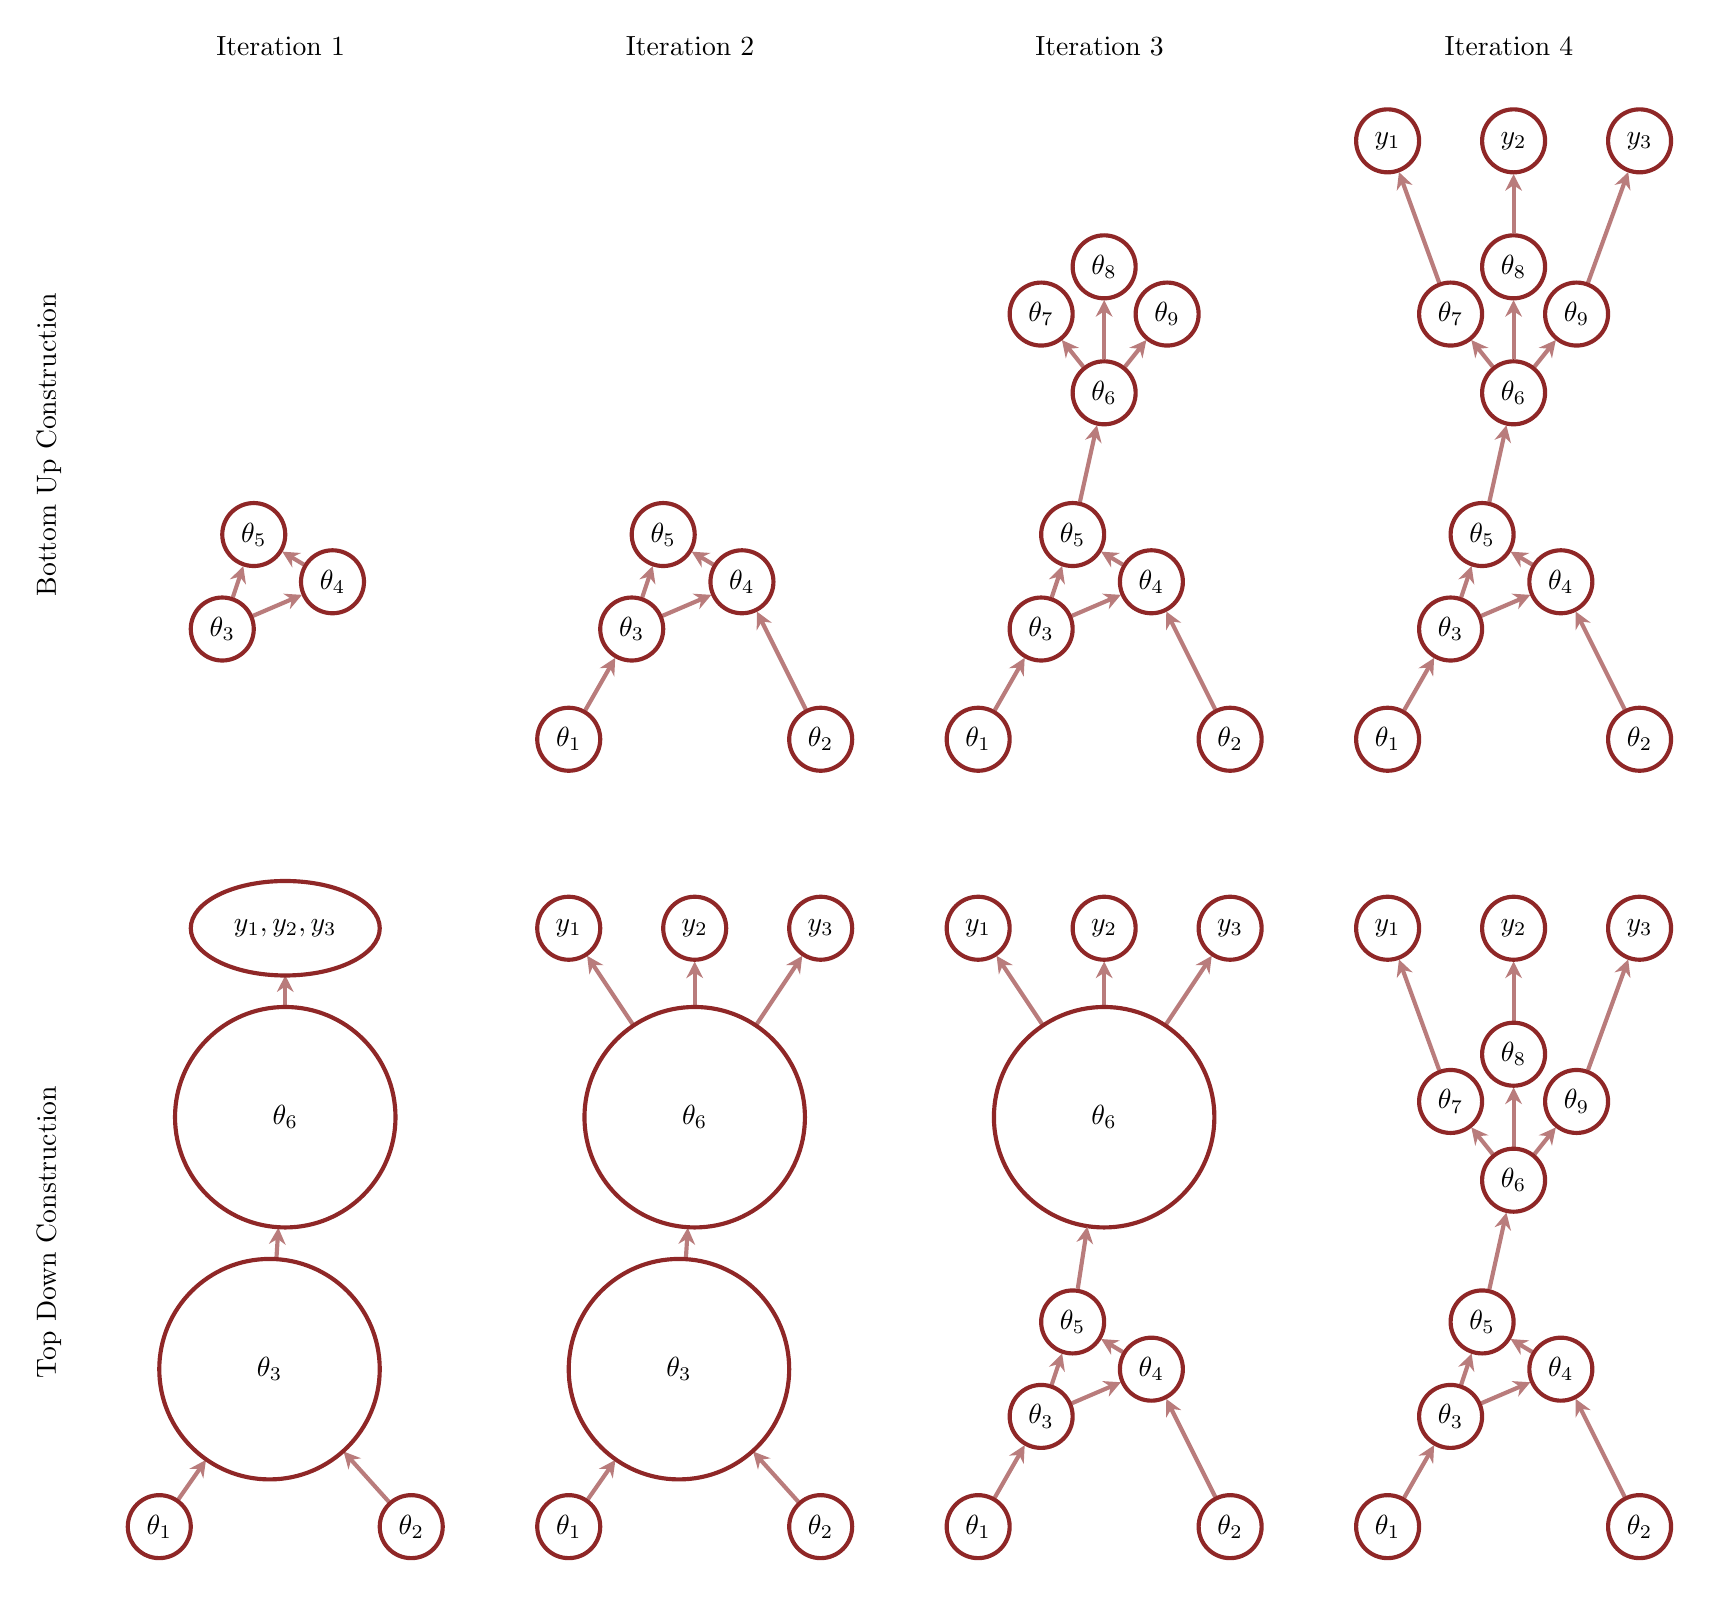
\begin{tikzpicture}[scale=0.2, thick]

  \pgfmathsetmacro{\r}{2}
  
  \node[align=center] at (0, 44) { Iteration 1 };
  \node[align=center] at (26, 44) { Iteration 2 };
  \node[align=center] at (52, 44) { Iteration 3 };
  \node[align=center] at (78, 44) { Iteration 4 };

  \node[align=center, rotate=90] at (-15, 19) { Bottom Up Construction };
  \node[align=center, rotate=90] at (-15, {19 - 50}) { Top Down Construction };
  
  \begin{scope}[shift={(0, 0)}]
    \draw[white] (-12, -4) rectangle (12, 42);
  
    \coordinate (A) at (-8, 0);
    \coordinate (B) at (8, 0);
    
    \coordinate (C) at (-4, 7);
    \coordinate (D) at (3, 10);
    \coordinate (E) at (-2, 13);
    
    \coordinate (F) at (0, 22);
    \coordinate (G) at (-4, 27);
    \coordinate (H) at (0, 30);
    \coordinate (I) at (4, 27);

    \coordinate (J) at (-8, 38);
    \coordinate (K) at (0, 38);
    \coordinate (L) at (8, 38);
    
    \foreach \B/\E in {C/D, C/E, D/E} {
      \draw[-{Stealth[length=6pt, width=6pt]}, shorten <=12.1, shorten >=12, color=mid, line width=1.5] (\B) -- (\E);
    }

    \filldraw[fill=white, draw=dark, line width=1.5] (C) circle (\r)
    node[color=black] { $\theta_{3}$ };
    
    \filldraw[fill=white, draw=dark, line width=1.5] (D) circle (\r)
    node[color=black] { $\theta_{4}$ };
    
    \filldraw[fill=white, draw=dark, line width=1.5] (E) circle (\r) 
    node[color=black] { $\theta_{5}$ };

  \end{scope}
  
  \begin{scope}[shift={(26, 0)}]
    \draw[white] (-12, -4) rectangle (12, 42);
  
    \coordinate (A) at (-8, 0);
    \coordinate (B) at (8, 0);
    
    \coordinate (C) at (-4, 7);
    \coordinate (D) at (3, 10);
    \coordinate (E) at (-2, 13);
    
    \coordinate (F) at (0, 22);
    \coordinate (G) at (-4, 27);
    \coordinate (H) at (0, 30);
    \coordinate (I) at (4, 27);

    \coordinate (J) at (-8, 38);
    \coordinate (K) at (0, 38);
    \coordinate (L) at (8, 38);
    
    \foreach \B/\E in {A/C, B/D, C/D, C/E, D/E} {
      \draw[-{Stealth[length=6pt, width=6pt]}, shorten <=12.1, shorten >=12, color=mid, line width=1.5] (\B) -- (\E);
    }

    \filldraw[fill=white, draw=dark, line width=1.5] (A) circle (\r)
    node[color=black] { $\theta_{1}$ };

    \filldraw[fill=white, draw=dark, line width=1.5] (B) circle (\r)
    node[color=black] { $\theta_{2}$ };

    \filldraw[fill=white, draw=dark, line width=1.5] (C) circle (\r)
    node[color=black] { $\theta_{3}$ };
    
    \filldraw[fill=white, draw=dark, line width=1.5] (D) circle (\r)
    node[color=black] { $\theta_{4}$ };
    
    \filldraw[fill=white, draw=dark, line width=1.5] (E) circle (\r) 
    node[color=black] { $\theta_{5}$ };

  \end{scope}
  
  \begin{scope}[shift={(52, 0)}]
    \draw[white] (-12, -4) rectangle (12, 42);
  
    \coordinate (A) at (-8, 0);
    \coordinate (B) at (8, 0);
    
    \coordinate (C) at (-4, 7);
    \coordinate (D) at (3, 10);
    \coordinate (E) at (-2, 13);
    
    \coordinate (F) at (0, 22);
    \coordinate (G) at (-4, 27);
    \coordinate (H) at (0, 30);
    \coordinate (I) at (4, 27);

    \coordinate (J) at (-8, 38);
    \coordinate (K) at (0, 38);
    \coordinate (L) at (8, 38);
    
    \foreach \B/\E in {A/C, B/D, C/D, C/E, D/E, E/F, F/G, F/H, F/I} {
      \draw[-{Stealth[length=6pt, width=6pt]}, shorten <=12.1, shorten >=12, color=mid, line width=1.5] (\B) -- (\E);
    }

    \filldraw[fill=white, draw=dark, line width=1.5] (A) circle (\r)
    node[color=black] { $\theta_{1}$ };

    \filldraw[fill=white, draw=dark, line width=1.5] (B) circle (\r)
    node[color=black] { $\theta_{2}$ };

    \filldraw[fill=white, draw=dark, line width=1.5] (C) circle (\r)
    node[color=black] { $\theta_{3}$ };
    
    \filldraw[fill=white, draw=dark, line width=1.5] (D) circle (\r)
    node[color=black] { $\theta_{4}$ };
    
    \filldraw[fill=white, draw=dark, line width=1.5] (E) circle (\r) 
    node[color=black] { $\theta_{5}$ };
    
    \filldraw[fill=white, draw=dark, line width=1.5] (F) circle (\r)
    node[color=black] { $\theta_{6}$ };
      
    \filldraw[fill=white, draw=dark, line width=1.5] (G) circle (\r)
    node[color=black] { $\theta_{7}$ };

    \filldraw[fill=white, draw=dark, line width=1.5] (H) circle (\r)
    node[color=black] { $\theta_{8}$ };

    \filldraw[fill=white, draw=dark, line width=1.5] (I) circle (\r)
    node[color=black] { $\theta_{9}$ };

  \end{scope}
  
  \begin{scope}[shift={(78, 0)}]
    \draw[white] (-12, -4) rectangle (12, 42);
  
    \coordinate (A) at (-8, 0);
    \coordinate (B) at (8, 0);
    
    \coordinate (C) at (-4, 7);
    \coordinate (D) at (3, 10);
    \coordinate (E) at (-2, 13);
    
    \coordinate (F) at (0, 22);
    \coordinate (G) at (-4, 27);
    \coordinate (H) at (0, 30);
    \coordinate (I) at (4, 27);

    \coordinate (J) at (-8, 38);
    \coordinate (K) at (0, 38);
    \coordinate (L) at (8, 38);
    
    \foreach \B/\E in {A/C, B/D, C/D, C/E, D/E, E/F, F/G, F/H, F/I, G/J, H/K, I/L} {
      \draw[-{Stealth[length=6pt, width=6pt]}, shorten <=12.1, shorten >=12, color=mid, line width=1.5] (\B) -- (\E);
    }

    \filldraw[fill=white, draw=dark, line width=1.5] (A) circle (\r)
    node[color=black] { $\theta_{1}$ };

    \filldraw[fill=white, draw=dark, line width=1.5] (B) circle (\r)
    node[color=black] { $\theta_{2}$ };

    \filldraw[fill=white, draw=dark, line width=1.5] (C) circle (\r)
    node[color=black] { $\theta_{3}$ };
    
    \filldraw[fill=white, draw=dark, line width=1.5] (D) circle (\r)
    node[color=black] { $\theta_{4}$ };
    
    \filldraw[fill=white, draw=dark, line width=1.5] (E) circle (\r) 
    node[color=black] { $\theta_{5}$ };
    
    \filldraw[fill=white, draw=dark, line width=1.5] (F) circle (\r)
    node[color=black] { $\theta_{6}$ };
      
    \filldraw[fill=white, draw=dark, line width=1.5] (G) circle (\r)
    node[color=black] { $\theta_{7}$ };

    \filldraw[fill=white, draw=dark, line width=1.5] (H) circle (\r)
    node[color=black] { $\theta_{8}$ };

    \filldraw[fill=white, draw=dark, line width=1.5] (I) circle (\r)
    node[color=black] { $\theta_{9}$ };
    
    \filldraw[fill=white, draw=dark, line width=1.5] (J) circle (\r)
    node[color=black] { $y_{1}$ };
 
    \filldraw[fill=white, draw=dark, line width=1.5] (K) circle (\r)
    node[color=black] { $y_{2}$ };
    
    \filldraw[fill=white, draw=dark, line width=1.5] (L) circle (\r)
    node[color=black] { $y_{3}$ };

  \end{scope}

  \begin{scope}[shift={(0, -50)}]
    \draw[white] (-12, -4) rectangle (12, 42);
  
    \coordinate (A) at (-8, 0);
    \coordinate (B) at (8, 0);
    
    \coordinate (C) at (-1, 10);
    
    \coordinate (F) at (0, 26);

    \coordinate (J) at (0, 38);
    
    \foreach \B/\E in {F/J} {
      \draw[-{Stealth[length=6pt, width=6pt]}, shorten <=12.1, shorten >=17, color=mid, line width=1.5] (\B) -- (\E);
    }
   
    \foreach \B/\E in {A/C, B/C, C/F} {
      \draw[-{Stealth[length=6pt, width=6pt]}, shorten <=12.1, shorten >=40, color=mid, line width=1.5] (\B) -- (\E);
    }

    \filldraw[fill=white, draw=dark, line width=1.5] (A) circle (\r)
    node[color=black] { $\theta_{1}$ };

    \filldraw[fill=white, draw=dark, line width=1.5] (B) circle (\r)
    node[color=black] { $\theta_{2}$ };

    \filldraw[fill=white, draw=dark, line width=1.5] (C) circle (7)
    node[color=black] { $\theta_{3}$ };
    
    \filldraw[fill=white, draw=dark, line width=1.5] (F) circle (7)
    node[color=black] { $\theta_{6}$ };
    
    \filldraw[fill=white, draw=dark, line width=1.5] (J) circle [x radius={3 * \r}, y radius={1.5 * \r}]
    node[color=black] { $y_{1}, y_{2}, y_{3}$ };

  \end{scope}
    
  \begin{scope}[shift={(26, -50)}]
    \draw[white] (-12, -4) rectangle (12, 42);
  
    \coordinate (A) at (-8, 0);
    \coordinate (B) at (8, 0);
    
    \coordinate (C) at (-1, 10);
    
    \coordinate (F) at (0, 26);

    \coordinate (J) at (-8, 38);
    \coordinate (K) at (0, 38);
    \coordinate (L) at (8, 38);
    
    \foreach \B/\E in {F/J, F/K, F/L} {
      \draw[-{Stealth[length=6pt, width=6pt]}, shorten <=12.1, shorten >=12, color=mid, line width=1.5] (\B) -- (\E);
    }
   
    \foreach \B/\E in {A/C, B/C, C/F} {
      \draw[-{Stealth[length=6pt, width=6pt]}, shorten <=12.1, shorten >=40, color=mid, line width=1.5] (\B) -- (\E);
    }

    \filldraw[fill=white, draw=dark, line width=1.5] (A) circle (\r)
    node[color=black] { $\theta_{1}$ };

    \filldraw[fill=white, draw=dark, line width=1.5] (B) circle (\r)
    node[color=black] { $\theta_{2}$ };

    \filldraw[fill=white, draw=dark, line width=1.5] (C) circle (7)
    node[color=black] { $\theta_{3}$ };
    
    \filldraw[fill=white, draw=dark, line width=1.5] (F) circle (7)
    node[color=black] { $\theta_{6}$ };
    
    \filldraw[fill=white, draw=dark, line width=1.5] (J) circle (\r)
    node[color=black] { $y_{1}$ };
 
    \filldraw[fill=white, draw=dark, line width=1.5] (K) circle (\r)
    node[color=black] { $y_{2}$ };
    
    \filldraw[fill=white, draw=dark, line width=1.5] (L) circle (\r)
    node[color=black] { $y_{3}$ };

  \end{scope}

  \begin{scope}[shift={(52, -50)}]
    \draw[white] (-12, -4) rectangle (12, 42);
  
    \coordinate (A) at (-8, 0);
    \coordinate (B) at (8, 0);
    
    \coordinate (C) at (-4, 7);
    \coordinate (D) at (3, 10);
    \coordinate (E) at (-2, 13);
    
    \coordinate (F) at (0, 26);

    \coordinate (J) at (-8, 38);
    \coordinate (K) at (0, 38);
    \coordinate (L) at (8, 38);
    
    \foreach \B/\E in {A/C, B/D, C/D, C/E, D/E, F/J, F/K, F/L} {
      \draw[-{Stealth[length=6pt, width=6pt]}, shorten <=12.1, shorten >=12, color=mid, line width=1.5] (\B) -- (\E);
    }

    \filldraw[fill=white, draw=dark, line width=1.5] (A) circle (\r)
    node[color=black] { $\theta_{1}$ };

    \filldraw[fill=white, draw=dark, line width=1.5] (B) circle (\r)
    node[color=black] { $\theta_{2}$ };

    \filldraw[fill=white, draw=dark, line width=1.5] (C) circle (\r)
    node[color=black] { $\theta_{3}$ };
    
    \filldraw[fill=white, draw=dark, line width=1.5] (D) circle (\r)
    node[color=black] { $\theta_{4}$ };
    
    \filldraw[fill=white, draw=dark, line width=1.5] (E) circle (\r) 
    node[color=black] { $\theta_{5}$ };
    
    \filldraw[fill=white, draw=dark, line width=1.5] (F) circle (7)
    node[color=black] { $\theta_{6}$ };
    
    \filldraw[fill=white, draw=dark, line width=1.5] (J) circle (\r)
    node[color=black] { $y_{1}$ };
 
    \filldraw[fill=white, draw=dark, line width=1.5] (K) circle (\r)
    node[color=black] { $y_{2}$ };
    
    \filldraw[fill=white, draw=dark, line width=1.5] (L) circle (\r)
    node[color=black] { $y_{3}$ };

    \foreach \B/\E in {E/F} {
      \draw[-{Stealth[length=6pt, width=6pt]}, shorten <=12.1, shorten >=40, color=mid, line width=1.5] (\B) -- (\E);
    }

  \end{scope}
  
  \begin{scope}[shift={(78, -50)}]
    \draw[white] (-12, -4) rectangle (12, 42);
  
    \coordinate (A) at (-8, 0);
    \coordinate (B) at (8, 0);
    
    \coordinate (C) at (-4, 7);
    \coordinate (D) at (3, 10);
    \coordinate (E) at (-2, 13);
    
    \coordinate (F) at (0, 22);
    \coordinate (G) at (-4, 27);
    \coordinate (H) at (0, 30);
    \coordinate (I) at (4, 27);

    \coordinate (J) at (-8, 38);
    \coordinate (K) at (0, 38);
    \coordinate (L) at (8, 38);
    
    \foreach \B/\E in {A/C, B/D, C/D, C/E, D/E, E/F, F/G, F/H, F/I, G/J, H/K, I/L} {
      \draw[-{Stealth[length=6pt, width=6pt]}, shorten <=12.1, shorten >=12, color=mid, line width=1.5] (\B) -- (\E);
    }

    \filldraw[fill=white, draw=dark, line width=1.5] (A) circle (\r)
    node[color=black] { $\theta_{1}$ };

    \filldraw[fill=white, draw=dark, line width=1.5] (B) circle (\r)
    node[color=black] { $\theta_{2}$ };

    \filldraw[fill=white, draw=dark, line width=1.5] (C) circle (\r)
    node[color=black] { $\theta_{3}$ };
    
    \filldraw[fill=white, draw=dark, line width=1.5] (D) circle (\r)
    node[color=black] { $\theta_{4}$ };
    
    \filldraw[fill=white, draw=dark, line width=1.5] (E) circle (\r) 
    node[color=black] { $\theta_{5}$ };
    
    \filldraw[fill=white, draw=dark, line width=1.5] (F) circle (\r)
    node[color=black] { $\theta_{6}$ };
      
    \filldraw[fill=white, draw=dark, line width=1.5] (G) circle (\r)
    node[color=black] { $\theta_{7}$ };

    \filldraw[fill=white, draw=dark, line width=1.5] (H) circle (\r)
    node[color=black] { $\theta_{8}$ };

    \filldraw[fill=white, draw=dark, line width=1.5] (I) circle (\r)
    node[color=black] { $\theta_{9}$ };
    
    \filldraw[fill=white, draw=dark, line width=1.5] (J) circle (\r)
    node[color=black] { $y_{1}$ };
 
    \filldraw[fill=white, draw=dark, line width=1.5] (K) circle (\r)
    node[color=black] { $y_{2}$ };
    
    \filldraw[fill=white, draw=dark, line width=1.5] (L) circle (\r)
    node[color=black] { $y_{3}$ };

  \end{scope}

\end{tikzpicture}

\end{document}  